\documentclass[10pt]{article}

% Preamble

\usepackage{amsmath,amsfonts,amssymb}
\usepackage[mathscr]{euscript}
%\usepackage[mathcal]{euscript}
\usepackage{mathrsfs}
\usepackage{graphicx}
\usepackage{float}
\usepackage{bbm}
\usepackage{braket}
\usepackage{tikz-feynman}
\usepackage{simpler-wick}
\usepackage{cancel}
\usepackage{stackengine}
\usepackage{slashed}
\usepackage{caption}
\usepackage{pgfplots}

\newcommand{\bigzero}{\mbox{\normalfont\Large\bfseries 0}}

\title{Lectures Notes For \\ An Introduction to Conformal Field Theory \\ A Course Given By Dr. Tobias Osborne} 
\author{Transcribed by Dr. Alexander V. St. John}

% The Document

\begin{document}

\maketitle

\clearpage

\section*{Lecture 1: Introduction to Conformal Field Theory}
\label{sec: lec1}

\noindent Recommended references:

\begin{itemize}
\item \textit{A Mathematical Introduction to Conformal Field Theory} by Schottenloher.
\item \textit{Applied Conformal Field Theory}, hep-th/9108028, by Ginsparg.
\item \textit{Conformal Field Theory} (``Yellow Book'') by Francesco, Mathieu, Senechal.
\end{itemize}

\noindent Why study conformal field theory (CFT)?

\begin{itemize}
\item CFT provides a good description of systems at or near criticality.
\item CFTs are the only true quantum field theories (QFTs), since they are cutoff-independent. One can think of QFTs as perturbations of CFTs. CFTs correspond to renormalization groups of fixed points, which dominate an effective theory at or near criticality.
\item CFTs can be made, by and large, mathematically rigorous, at least in $(1+1)$-dimensional theories. There are three major competing mathematical descriptions for CFT, and advances are being made towards a single, unifying description.
\end{itemize}

\noindent Prerequisites for this material:

\begin{itemize}
\item Advanced quantum mechanics
	\subitem E.g, many-body theory and Fock spaces.
\item Classical field theory
	\subitem E.g., symplectic geometry.
\item Quantum field theory.
\item Advanced quantum field theory.
\end{itemize}

\noindent What is CFT?

\begin{itemize}
\item A \textit{conformal field theory} is a field theory, quantum or classical, that is invariant, or symmetric, under a group of transformations called the \textit{conformal group} $G$.
\item In a classical field theory, this means that the equations of motion are left invariant.
\item In a quantum field theory, this means that, by Wigner's theorem, there is a projective unitary representation of the group $G$. In other words, symmetries, or transformations, that leave the transition amplitude invariant, are realized, up to a phase, by (anti)unitary operators.
\end{itemize}

\subsection*{Conformal Transformations in $d$ Dimensions}

\noindent Let $M = \mathbb{R}^{p,q}$ be a manifold $\mathbb{R}^d$, where $d = p+q$, and $p,q \in \mathbb{Z}_{\ge 0}$. To this manifold, assign the metric

\begin{equation}
g_{\mu\nu} \equiv \eta_{\mu\nu} = \text{diag} (1,1,\dots,1,-1,-1,\dots,-1)
\end{equation}

\noindent With the first $p$ entries equal to one, and the last $q$ entries equal to minus one. Note that this is not necessarily a Riemannian metric, since the signature can be negative. We have a few cases of interest for this metric

\begin{itemize}
\item $p=d$ , Riemannian.
\item $p = d-1$, $q=1$, Lorentz.
\item $q > 1$, e.g., $q=2$, AdS-CFT correspondence.
\end{itemize}

\noindent A conformal transformation leaves the metric invariant up to a scale factor. \\

\noindent Consider a smooth change of coordinates

\begin{equation}
x \rightarrow x' = x' (x) \text{ , with } x = (x^1, x^2, \dots, x^p, x^{p+1}, \dots, x^{p+q})
\end{equation}

\noindent Such that the metric, a type-$(2,0)$ tensor, undergoes an \textit{active coordinate} transformation as

\begin{equation}
g_{\mu\nu} (x) \rightarrow g'_{\mu\nu} (x') \equiv \frac{\partial x^\alpha}{\partial x'^\mu} \frac{\partial x^\beta}{\partial x'^\nu} g_{\alpha \beta} (x') 
\end{equation}

\noindent And then impose the condition

\begin{equation}
g'_{\mu\nu} (x') = \Omega (x') g_{\mu\nu} (x').
\end{equation}

\noindent Where $\Omega(x) > 0$ is the (local) scale factor. Note that if the scale factor is zero, then we have a singularity, which we will discuss later. A transformation that obeys the last line is called \textit{conformal}, and these transformations preserve angles

\begin{equation}
\angle \theta = \frac{g_{\mu\nu} u^\mu v^\nu}{\sqrt{(g_{\mu\nu} u^\mu v^\nu)^2}}.
\end{equation}

\noindent The \textit{conformal group} of a manifold M is denoted by $\text{Conf}(M)$, and is the connected component of the group of all conformal transformations of $M$ containing the identity, in a compact, open topology. \\

\noindent So, in a quantum conformal field theory, we are looking for a Hilbert space $\mathcal{H}$ and a projective unitary representation of the group $G$ for \textit{local} QFTs

\begin{equation}
G \rightarrow \pi (G).
\end{equation}

\noindent This is unexpectedly nontrivial, and makes for a very rich field of study, since there is a tension between knowing the unitary representations of symmetries and demanding that the representation is locally implementable. \\

\noindent To classify the conformal group on our chosen manifold $G = \text{Conf} (\mathbb{R}^{p,q})$, consider an infinitesimal conformal (active coordinate) transformation on the spacetime coordinates

\begin{equation}
x^\mu \rightarrow x'^\mu = x^\mu +  \epsilon^\mu (x)
\end{equation}

\noindent Which must leave the metric invariant up to the scale factor $\Omega(x)$. This places constraints on $\epsilon$ (\textbf{Exercise}) \\

\begin{equation}
g_{\mu\nu} \rightarrow g'_{\mu\nu} = g_{\mu\nu} + (\partial_\mu \epsilon_\nu + \partial_\nu \epsilon_\mu) + \mathcal{O} (\epsilon^2).
\end{equation}

\noindent To satisfy the constraint placed by conformal invariance on the metric (c.f., $g_{\mu\nu} \rightarrow g'_{\mu\nu} (x') = \Omega(x') g_{\mu\nu} (x')$), as well as the constraint that the conformally transformed metric is still proptional to the diagonal flat spacetime metric $g'_{\mu\nu} \propto \eta_{\mu\nu}$, we must have that the second term is also diagonal, proportional to $\eta_{\mu\nu}$

\begin{align}
(\partial_\mu \epsilon_\nu + \partial_\nu \epsilon_\mu) &\propto \eta_{\mu\nu} \\
\implies (\partial_\mu \epsilon_\nu + \partial_\nu \epsilon_\mu) &= \text{constant} \cdot \eta_{\mu\nu}
\end{align}

\noindent Take the trace of each side, set $\mu=\nu$, and solve for the constant

\begin{equation}
\text{constant} = \frac{2 (\partial \cdot \epsilon)}{d}
\end{equation}

\noindent So, the conformal transformation on the metric reads, tossing out higher order terms,

\begin{equation}
g'_{\mu\nu} = g_{\mu\nu} + \frac{2 (\partial \cdot \epsilon)}{d} g_{\mu\nu}.
\end{equation}

\noindent And substituting into the proportionality relation from above, we have

\begin{equation}
(\partial_\mu \epsilon_\nu + \partial_\nu \epsilon_\mu) = \frac{2}{d} (\partial \cdot \epsilon) \eta_{\mu\nu}.
\end{equation}

\noindent Combining this with the conformal transformation of the metric and comparing to the metric transformation law, we get that the scale factor $\Omega(x)$ for the conformal transformation of the spacetime metric is 

\begin{equation}
\Omega(x) = 1+\frac{2}{d} (\partial \cdot \epsilon).
\end{equation}

\noindent Then it follows from $(\partial_\mu \epsilon_\nu + \partial_\nu \epsilon_\mu) = \frac{2}{d} (\partial \cdot \epsilon) \eta_{\mu\nu}$ , expanding and equating mixed partial derivatives to third order, and we get $d^2$ partial differential equations of the form (\textbf{Exercise})

\begin{equation}
(\eta_{\mu\nu} \Box + (d-2) \partial_\mu \partial_\nu) (\partial \cdot \epsilon) = 0
\end{equation}

\noindent Where $\Box = \eta^{\mu\nu} \partial_\mu \partial_\nu$ is the d'Alembertian operator.

\subsubsection*{Classification of Infinitesimal Conformal Translations for $d>2$}

\noindent By examining the condition for $\epsilon$ and the $d^2$ equations

\begin{align}
(\partial_\mu \epsilon_\nu + \partial_\nu \epsilon_\mu) &= \frac{2}{d} (\partial \cdot \epsilon) \eta_{\mu\nu} \\
(\eta_{\mu\nu} \Box + (d-2) \partial_\mu \partial_\nu) (\partial \cdot \epsilon) &= 0
\end{align}

\noindent We find that third order derivatives of $\epsilon(x)$ vanish and $\epsilon(x)$ is at most quadratic. \\

\noindent This leaves four types of infinitesimal transformations, defined via $\epsilon$, allowable in a conformal transformation: one constant, two linear, and one quadratic in spacetime coordinates.

\begin{enumerate}
\item Spacetime translations
	\subitem $\epsilon = a^\mu$.
\item Rotations
	\subitem  $\epsilon^\mu = \omega^\mu_{\,\,\nu} x^\nu$, $\omega$ antisymmetric.
\item Scale transformations
	\subitem $\epsilon^\mu = \lambda x^\mu$, $\lambda > 0$.
\item Special conformal transformations (SCT; inversion through a sphere)
	\subitem $\epsilon^\mu = b^\mu x^2 - 2 x^\mu (b \cdot x)$.
\end{enumerate}

\noindent Note that Lorentz and Poincar\'e transformations are always subgroups of the conformal group, leaving the metric invariant. since $\omega$ corresponds to boosts and Euclidean affine rotations complete the Poincar\'e group. \\

\noindent \textbf{Theorem} \\

\noindent Every conformal transformation that acts on an connected subset of Minkowski space, including the whole space itself, $\varphi : \, U \subset \mathbb{R}^{p,q}$, where $p+q > 2$, is a composition of 

\begin{itemize}
\item a translation
	\subitem $x^\mu \rightarrow x^\mu + a^\mu$, where $a \in \mathbb{R}^d$,
\item an orthogonal transformation (rotation)
	\subitem $x \rightarrow \Lambda x$, where $\Lambda \in O(p,q)$,
\item a dilation (scale)
	\subitem $x^\mu \rightarrow \lambda x^\mu$, where $\lambda \in \mathbb{R}^+$,
\item and an SCT
	\subitem $x \rightarrow \frac{x^\mu - b^\mu x^2 }{1-2b \cdot x + b^2 x^2}$, where $b \in \mathbb{R}^q$.
\end{itemize}

\noindent Note that it is possible to find a vector $b$ such that the denominator is equal to zero, the SCT is not invertible, and this is no longer a group. Also note that if we don't compactify the space and include $\infty$ as a point available to the conformal transformation, the group becomes significantly smaller and more constrained. \\

\subsubsection*{Classification of Infinitesimal Conformal Translations for $d=2$}

\noindent If $d=2$, the spacetime metric becomes the identity

\begin{equation}
g_{\mu\nu} = \delta_{\mu\nu}
\end{equation}

\noindent And $(\partial_\mu \epsilon_\nu + \partial_\nu \epsilon_\mu) = \frac{2}{d} (\partial \cdot \epsilon) \eta_{\mu\nu}$ becomes the Cauchy-Riemann equations and $\epsilon(x)$ is complex-valued, complex-differentiable, and analytic

\begin{equation}
\partial_1 \epsilon_1 = \partial_2 \epsilon_2 \text{ and } \partial_1 \epsilon_2 = - \partial_2 \epsilon_1.
\end{equation}

\noindent Introduce the complex coordinates

\begin{equation}
z = x^1 + i x^2 \text{ and } \bar{z} = x^1 - i x^2.
\end{equation}

\noindent Then we can complexify $\epsilon$ as

\begin{equation}
\epsilon(z) = \epsilon^1 + i \epsilon^2 \text{ and } \bar{\epsilon}({\bar{z}}) = \epsilon^1 - i \epsilon^2.
\end{equation}

\noindent Two-dimensional global, gotten via exponentiation of an infinitesimal transformation, conformal transformations correspond to \textit{entire} (no singularities, invertible everywhere), \textit{holomorphic} functions $z \rightarrow f(z)$ with holomorphic inverses $f^{-1} (z)$. The only allowable form for a conformal transformation that corresponds to an entire, holomorphic function is linear in the complex coordinates

\begin{equation}
f(z) = \alpha z + \beta, \text{ where } \alpha, \beta \in \mathbb{C}.
\end{equation}

\noindent We may expect a larger group of symmetries with entirety and holomorphism enforced, since the space seems less constrained, but this actually constrains the space more and the group becomes smaller. So, if we were to not compactify, and add infinity as a point, as we demonstrated, the conformal space becomes linear and boring: only rotations and scaling are allowed.\\

\noindent To include this complex representation of the spacetime coordinates, we \textit{extend} our manifold to the complex numbers $\mathbb{C}$ and compactify complex space to a Riemann sphere $\mathbb{C} \cup \{ \infty \}$ we get the proper space for the conformal transformations to act in

\begin{equation}
\mathbb{R}^{2,0} \rightarrow \mathbb{C} \rightarrow \mathbb{C} \cup \{\infty\} \rightarrow \text{Conf}(\mathbb{C} \cup \{\infty\} )
\end{equation}

\begin{figure}[H]
	\centering
	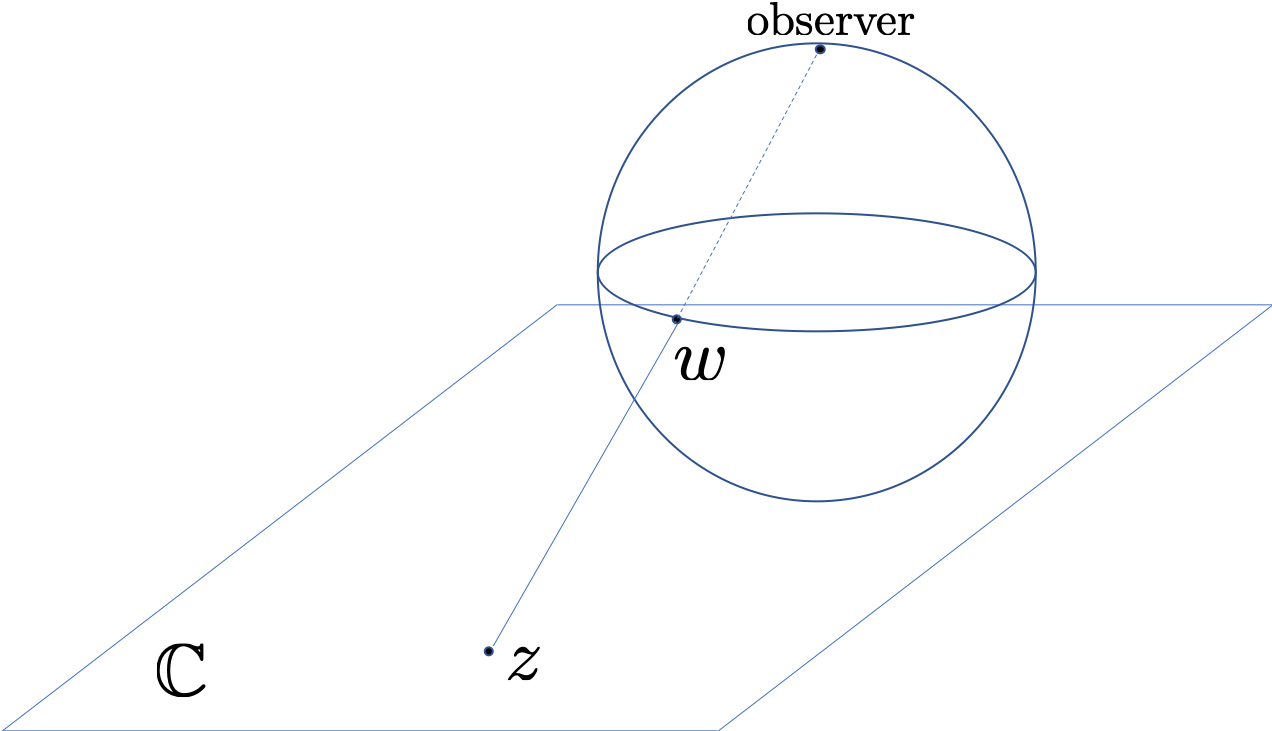
\includegraphics[width=3in]{images/riemann_sphere.png} 
\end{figure} 

\noindent Where the conformal group is

\begin{equation}
\text{Conf}(\mathbb{C} \cup \{ \infty \} ) = \Big{\{} f(z) = \frac{\alpha z + \beta}{\gamma z + \delta}; \, \alpha, \beta, \gamma, \delta \in \mathbb{C}, \alpha\delta - \beta \gamma \ne 0 \Big{\}}.
\end{equation}

\noindent This is also called the group of Moebius transformations, and is a slightly larger group of conformal transformations (symmetires), since we can map to and from infinity as a point. \\

\subsubsection*{Summary}

\noindent A conformal field theory is a local quantum field theory that is invariant under the conformal group, a set of transformations, a change in coordinates, that leave the metric invariant up to a scale factor. In different spacetime dimensions, the conformal group takes on significantly different forms. \\

\noindent The global conformal group in dimensions greater than two is comprised of translations, rotations, scaling, and special conformal transformations, as well as dimensions equal to two, as long as the space is compactified. If singularities are included, functions with poles are allowed, the symmetry gets larger.


\clearpage

\section*{Lecture 2: Local Conformal Transformations}
\label{sec: lec2}


\noindent In the last lecture we introduced global conformal transformations/symmetries of some manifold $M$ that form a (symmetry) group $G$ which can be promoted to a symmetry group of some quanutm system, where the kinematics of the system are described by a Hilbert space $\mathcal{H}$. The quantum system is said to be globally conformally invariant if these is some unitary representation, operators $U$ that act on the Hilbert space,

\begin{equation}
U: \,\, G \rightarrow U(\mathcal{H}).
\end{equation}

\noindent Recall that in the generalized Minkowski space $\mathbb{R}^{p,q}$, the structure of the group of global conformal transformations $G$ consists of compositions of translations, dilations, rotations(boosts), and special conformal transformations (SCTs). \\

\noindent Here we now study the case where $d=2$, which will expand our notion of what a symmetry is and will allow us to define local, infinitesimal conformal transformations. \\

\noindent For example, a global conformal transformation, a $1-1$ differentiable map from $\mathbb{R}^2 \rightarrow \mathbb{R}^2$, may consist of a dilation and a rotation and look like

\begin{figure}[H]
	\centering
	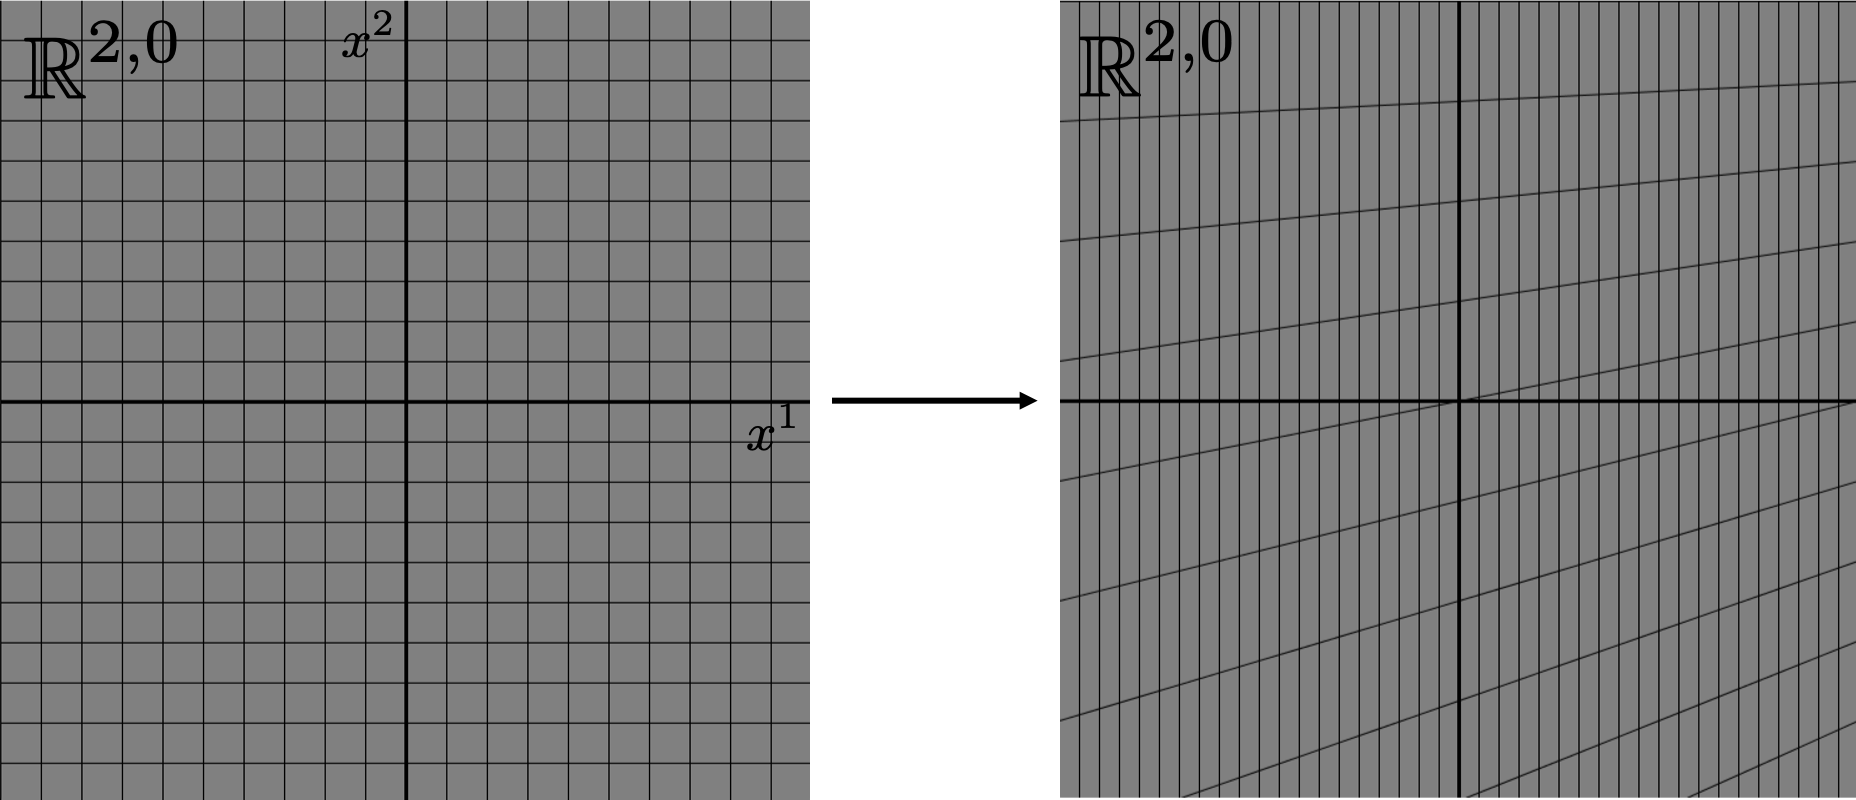
\includegraphics[width=4in]{images/global_conf_trans.png} 
\end{figure} 

\noindent For contrast, consider an infinitesimal conformal transformation $\text{id} + \epsilon X$, where $X=X(x)$ is a vector field, the derivative of a diffeomorphism, that acts on the two-dimensional Minkowski space as

\begin{figure}[H]
	\centering
	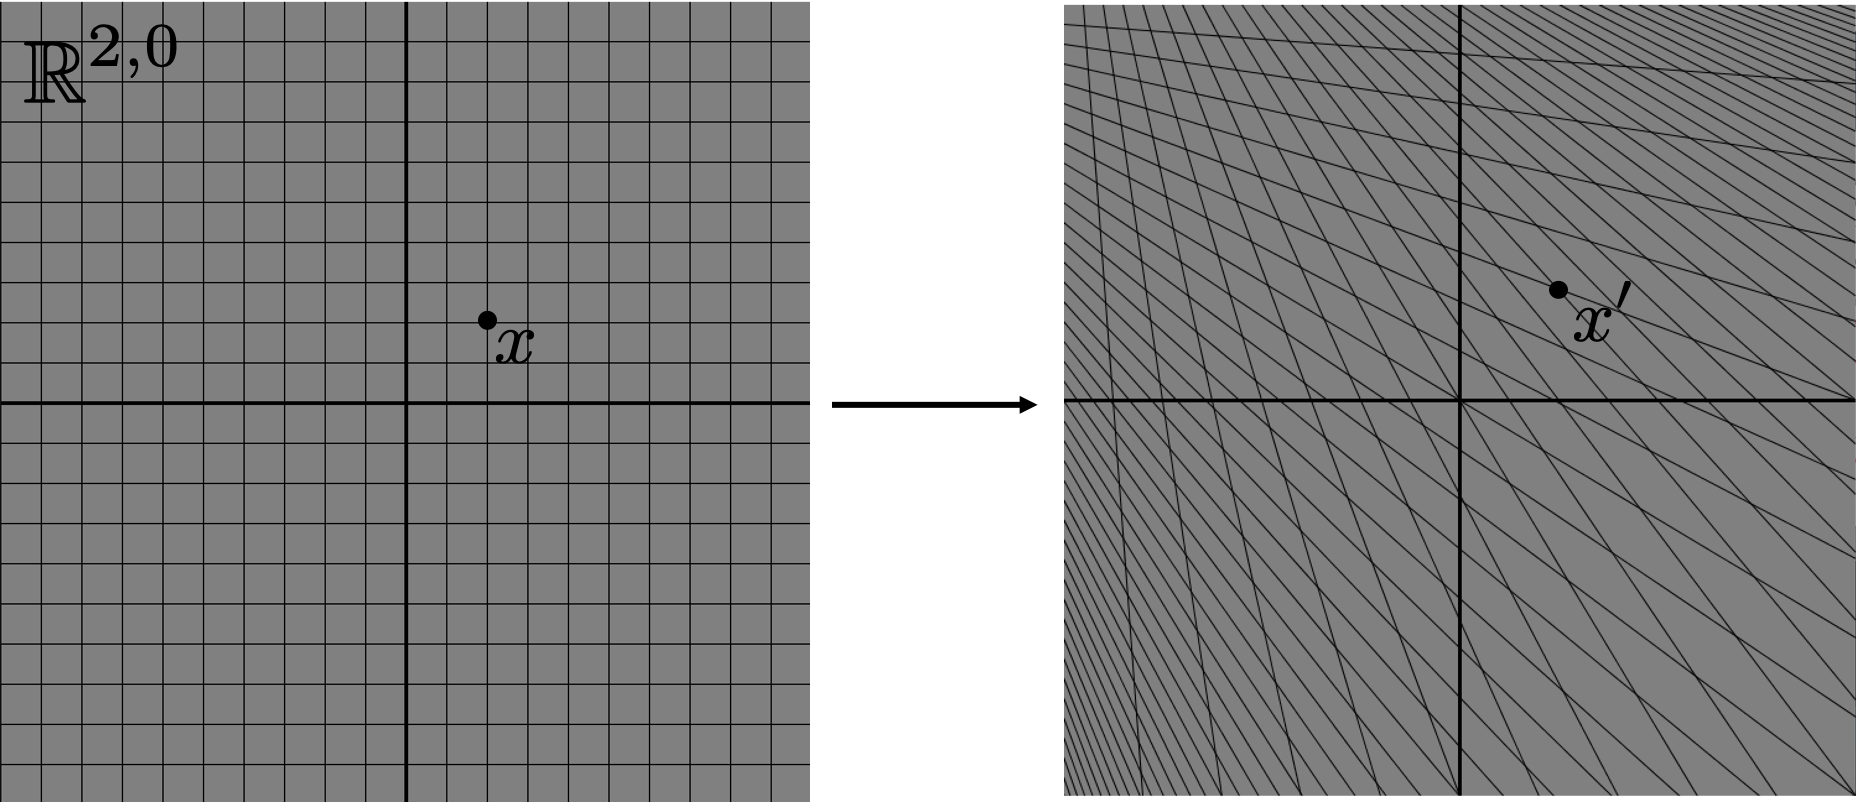
\includegraphics[width=4in]{images/inf_conf_trans.png} 
\end{figure} 

\noindent This transformation preserves all of the right angles in the untransformed Minkowski space, and the action is close to the identity, such that $|x-x'| \sim \mathcal{O}(\epsilon)$. The transformation $\text{id} + \epsilon X$ is conformal to first order in $\epsilon$, as is required by the definition of infinitesimal. \\

\noindent Although the vector field $X(x)$ is a generator of the infinitesimal conformal transformation, it does not necessarily define a global transformation via exponentiation, as it just may not be well defined globally.\\

\noindent To begin to make sense of this, consider in quantum mechanics, where we talk about quantum systems symmetric under a group $G$ with HIlbert space 

\begin{equation}
(\mathcal{H}, \,\, U: \, G \rightarrow U(\mathcal{H})).
\end{equation}

\noindent So, in quantum mechanics, we are reduced to finding these unitary representations of $G$. If $G$ is finite, it does not make sense to speak infinitesimally (e.g., one one-hundredth of a reflection). \\

\noindent We assume $G$ is a manifold, and then we may as well go as far to assume that $G$ is a Lie group with an associated Lie algebra $\mathfrak{g}$, which consists of vector fields that exponentiate to the Lie group. Then the quantum system is symmetric under the Lie algebra if you get a representation

\begin{equation}
(\mathcal{H}, \, \, \pi: \, \mathfrak{g} \rightarrow L(\mathcal{H}))
\end{equation}

\noindent Where $L(\mathcal{H})$ is the set of (bounded and unbounded) linear operators, and $\pi$ generates a unitary operator on the Hilbert space, such that $\pi(X)= e^{isX}$, $s\in \mathbb{R}$. \\

\noindent Note that for an infinite-dimensional group, (1) the operator $e^{isX}$ may not be continuous, and (2) the Lie algebra may not exponeniate to a Lie group, which we will encounter in conformal field theory. In other words, in contrast to when we used infinitesimal quanities to build global representations, we find that infinitesimal conformal transformations don't necessarily exponentiate to a group.\\

\noindent Therefore, in the infinitesimal case, we abandon looking for (full, continuous) unitary representations of the Lie group, and instead focus in on finding Hermitian representations that generate the Lie algebra. \\

\subsection*{Local algebra of infinitesimal conformal transformations}

\noindent Recall that for global conformal transformations, we have $z \rightarrow f(z)$, where $f$ is holomorphic with inverse $f^{-1}$. For infinitesimal $f$, this transformation, including the complex conjugate, becomes

\begin{equation}
z \rightarrow z + \epsilon (z) \text{ and } \bar{z} \rightarrow \bar{z} + \bar{\epsilon}(\bar{z})
\end{equation}

\noindent Where $\epsilon$ is a holomorphic function. A convenient choice of basis, which is infinite dimensional, is

\begin{equation}
\epsilon_n (z) = -\epsilon z^{n+1} \text{, where } n \in \mathbb{Z}.
\end{equation}

\noindent Given a diffeomorphism $[z \rightarrow z + \epsilon_n (z)] = e^{\epsilon \ell_n}$, the corresponding vector field tangent to every point in the manifold is defined by the operators

\begin{equation}
\ell_n \equiv - z^{n+1} \partial_z \text{ and } \bar{\ell}_n \equiv - \bar{z}^{n+1} \partial_{\bar{z}}.
\end{equation}

\noindent These differential operators form a basis, since they obey the commutation relations (\textbf{Exercise})

\begin{align}
[ \ell_m , \ell_n ] &= (m-n) \ell_{m+n} \\
[ \bar{\ell}_m, \bar{\ell}_n ] &= (m-n) \bar{\ell}_{m+n} \\
[\bar{\ell}_m , \ell_n ] &= 0.
\end{align}

\noindent They also as form a closed, infinite-dimensional Lie algebra $\forall m,n \in \mathbb{Z}$, called the Witt algebra $\text{WItt} = \mathcal{A} \oplus \bar{\mathcal{A}}$, where $\mathcal{A}$ is generated by $\{ \ell \}$, and $\bar{\mathcal{A}}$ is generated by $\{ \bar{\ell} \}$. Everything commutes in the basis, so the direct sum of the Witt algebra is justified. \\

\noindent The Witt algebra is generated infinitesimally, and could also be used to infinitiseimally generate a Lie group. This turns out to be true, but the Lie group is not the conformal group. \\

\noindent Which operators $\ell_n$ correspond to global transformations? \\

\noindent Consider a vector field 

\begin{equation}
v(z) = - \sum_{n=-\infty}^{\infty} v_n \ell_n = \sum_{n=-\infty}^{\infty} v_n z^{n+1} \partial_z.
\end{equation}

\noindent For this vector field to correspond to a global transformation, $v(z)$ must exponentiate to a holomorhpic map $f$, which is nonsingular in the limit as $z \rightarrow 0$. This places constraints on the coefficients of the vector field 

\begin{equation}
v_n = 0, \, n < -1.
\end{equation}

\noindent The inverse of the vector field must also exponentiate to a holomorphic map $f^{-1}$, which is nonsingular in the limit as $z \rightarrow \infty$ (e.g., exists on the Riemann sphere). This places the constraint on the coefficients of the vector field: 

\begin{equation}
v_n = 0, \, n>1.
\end{equation}

\noindent Note that if we demand holomorphism on the full complex plane without compactifying, the only allowed global transformations will be linear transformation (\textbf{Exercise}). By compactifying $\pm \infty$ as a point onto the Riemann sphere, we have more freedom in allowed global transformations. \\

\noindent With these constraints in place, we are left with three (six with complex conjugates) generators of infinitesimal global conformal transformations

\begin{equation}
\ell_{-1}, \ell_0 , \ell_1 \text{ and } \bar{\ell}_{-1}, \bar{\ell}_0, \bar{\ell}_1.
\end{equation}

\noindent The generators close to form a subalgebra under the commutator bracket $[,]$ defined above (\textbf{Exercise}), and generate thegroup of \textit{linear fractional (Moebius) transformations}, also known as the projective special linear group $\text{PSL}(2,\mathbb{C})$

\begin{equation}
z \rightarrow \frac{az + b}{c z + d}, \,\, ad-bc = 1.
\end{equation}

\noindent The set of global conformal transformations allowed in this basis are (\textbf{Exercise}), for $s \in \mathbb{R}$,

\begin{align}
&\text{Translation: } &e^{s \ell_{-1}} \equiv &\begin{pmatrix}1&-s \\ 0&1 \end{pmatrix} &\equiv z \rightarrow z - s \\
&\text{Dilation: } &e^{s (\ell_0 + \bar{\ell}_0)} \equiv &\begin{pmatrix}\lambda&0 \\ 0&\lambda^{-1} \end{pmatrix} &\equiv z \rightarrow e^{-s} \\
&\text{Rotation: } &e^{is (\bar{\ell}_0 - \ell_0)} \equiv &\begin{pmatrix}\text{exp}(i\frac{\theta}{2})&0 \\ 0&\text{exp}(-i\frac{\theta}{2}) \end{pmatrix} &\equiv z \rightarrow e^{is} \\
&\text{Special: } &e^{s \ell_1} \equiv &\begin{pmatrix}1&0 \\ c&1 \end{pmatrix} &\equiv z \rightarrow \frac{z}{1+sz}.
\end{align}

\noindent Note that for $\mathbb{R}^{d,0}$, $d>2$, the local transformations are also global! Also note that in one-dimensional spacetime, $(1,0)$ or $(0,1)$, conformal transformations are all monotonic increasing functions $\mathbb{R} \rightarrow \mathbb{R}$.

\subsection*{$d=2$ Minkowski space, $\mathbb{R}^{1,1}$}

\noindent The conformal group  of $\mathbb{R}^{1,1}$ is \textit{special}. \\

\noindent \textbf{Theorem:} \\

\noindent A smooth map $\varphi = (u,v) : \, M \rightarrow \mathbb{R}^{1,1}$ from a connected subset of $M \subset \mathbb{R}^{1,1}$ is conformal (pulls back metric to a scalar multiple of the diagonal metric), iff $u_x^2 > v_x^2$ and $u_x = v_y,\, u_y = v_x$ or $u_x = -v_y,\, u_y = -v_x$. \\

\begin{figure}[H]
	\centering
	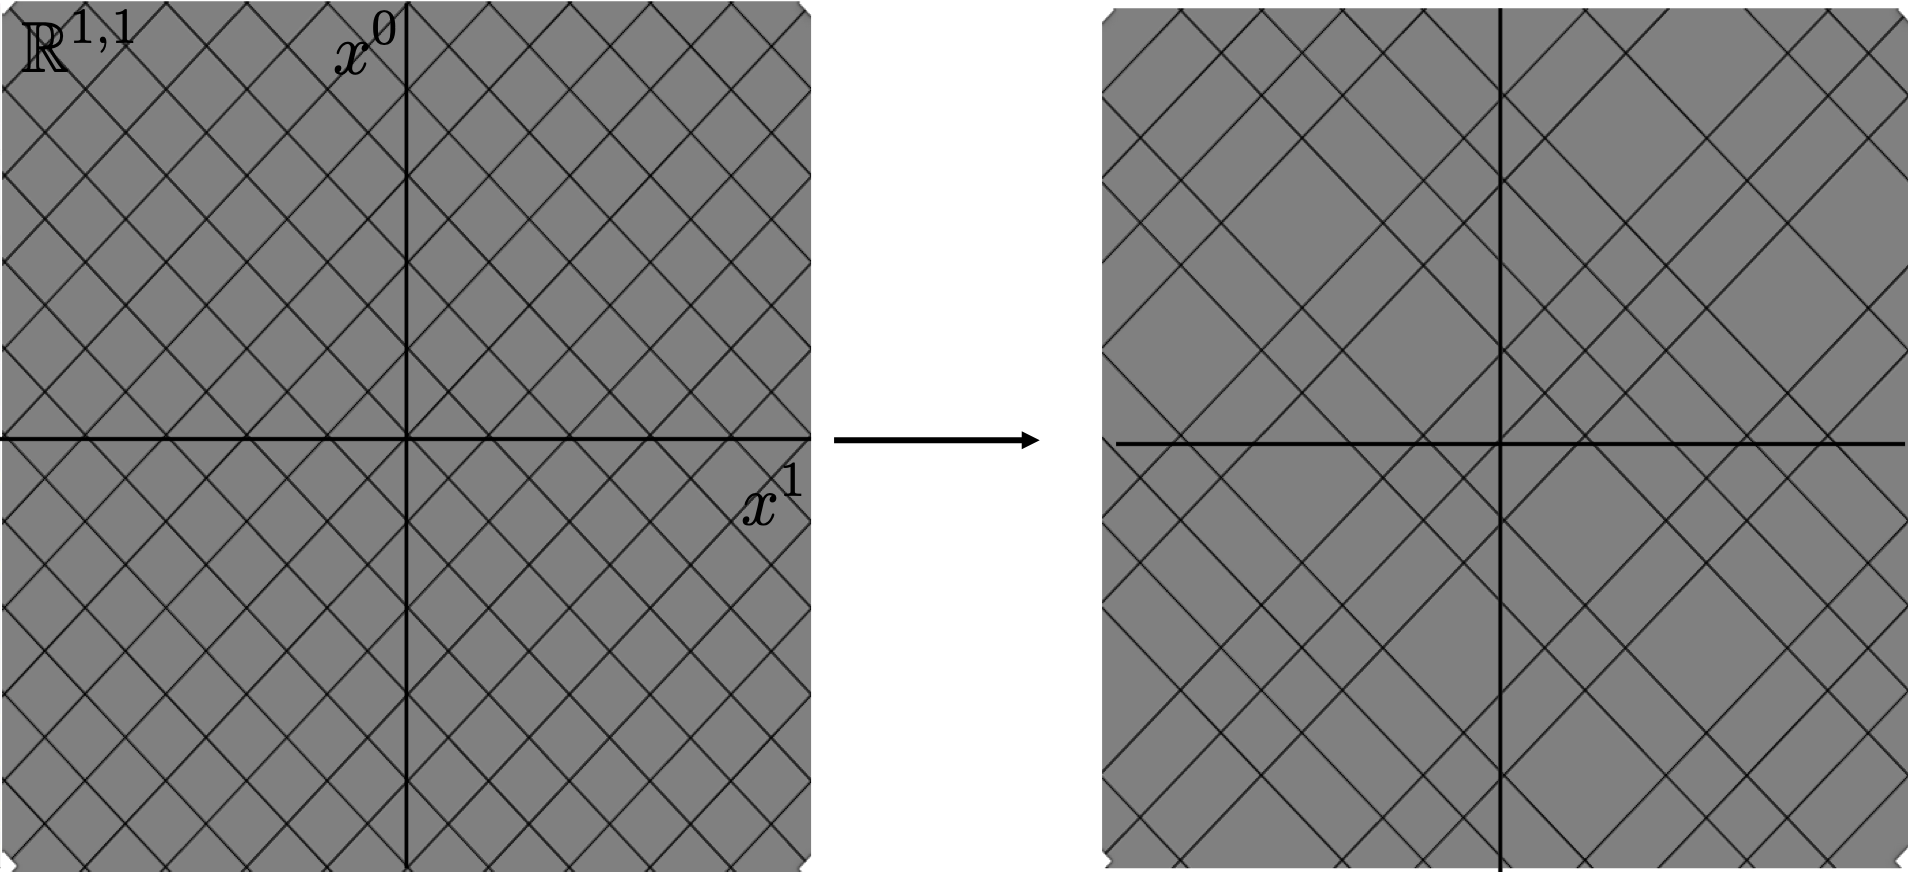
\includegraphics[width=4in]{images/conf_trans_lightcone.png} 
\end{figure} 

\noindent \textbf{Theorem:} \\

\noindent Consider an infinitely differentiable function on the real line $f \in C^\infty (\mathbb{R})$, and let $f_\pm \in C^\infty (\mathbb{R}^2, \mathbb{R})$, the infinitely differentiable functions from the real line to the real plane, be defined by $f_\pm (x,y) = f(x \pm y)$. Then the map 

\begin{align}
\Phi: \, C^\infty (\mathbb{R}) \times C^\infty (\mathbb{R}) &\rightarrow C^\infty (\mathbb{R}^2, \mathbb{R}^2) \\
(f,g) &\rightarrow \frac{1}{2} (f_+ + g_-, f_+ - g_- )
\end{align}

\noindent Has the following properties

\begin{itemize}
\item image($\Phi$) $= \{ (u,v): \, u_x = v_y, \, u_y, v_x \}$
\item $\Phi(f,g)$ is conformal iff $f'>0$ and $g' >0$ or $f'<0$ and $g'<0$
\item $\Phi$ is bijective iff $f$ and $g$ are bijective
\item $\Phi(f \circ h, g \circ k) = \Phi(f,g) \circ \Phi (h,k), \forall f,g,h,k \in C^\infty(\mathbb{R}) \equiv \Phi$ is a homomorphism.
\end{itemize}

\noindent The group of orientation-preserving transformations of $M=\mathbb{R}^{1,1}$ is isomorphic to 

\begin{equation}
(\text{Diff}_+ (\mathbb{R}) \times \text{Diff}_+ (\mathbb{R})) \cup (\text{Diff}_- (\mathbb{R}) \times \text{Diff}_- (\mathbb{R}))
\end{equation}

\noindent Which consists of the infinitely-differentiable orientation-preserving maps of $\mathbb{R}$, diffeomorphisms of $\mathbb{R}$. \\

\noindent It is convenient to compactify $\mathbb{R}^{1,1} \rightarrow S^{1,1} \subset \mathbb{R}^{2,0} \times \mathbb{R}^{0,2}$. Then the group of orientation-preserving transformations of $M=S^{1,1}$ is isomorphic to 

\begin{equation}
\text{Conf} (\mathbb{R}^{1,1}) \equiv (\text{Diff}_+ (S^1) \times \text{Diff}_+ (S^1)) \cup (\text{Diff}_- (S^1) \times \text{Diff}_- (S^1)).
\end{equation}

\noindent This is the definition of the conformal group of Minkowski space. Typically, we throw away the second part of the union, the $''-''$ reversing part, since it is the same as preserving with $z \rightarrow -z$, and focus on the infinite-dimensional subgroup $\text{Diff}_+ (S^1)$, which we call the \textit{chiral half} of the conformal group. This is admissable, since the symmetries of a quantum system can be understood by the symmetries of $\text{Diff}_+ (S^1)$, and the rest is easily gotten by tensor products to include the other light-cone axes. \\

\noindent In the next lecture, we will focus on which quantum systems are invariant under this infinite-dimensional group $\text{Diff}_+ (S^1)$ by going to the Lie algebra, which turns out to be isomorphic to the Witt algebra, in the Euclidean case. The unitary representations, gotten via infinitesimal generators, of $\text{Diff}_+ (S^1)$ will not be bounded below and are unstable. Therefore, \textit{projective} unitary representaitons will be required, and are classified by the \textit{central charge}.

\clearpage

\section*{Lecture 3: Classical Conformal Field Theory}
\label{sec: lec3}


\noindent We continue our discussion of systems that exhibit conformal symmetries. These symmetries are contained in the conformal group called $\text{Conf}(\mathbb{R}^{p,q})$, which is the connected component containing the identity of all conformal diffeomorphisms of the pseudo-Riemannian manifold $\mathbb{R}^{p,q}$. \\

\noindent We discussed the infinitesimal conformal transformation, which led to a Lie algebra, the Witt algebra, in $(1+1)$ and $(2,0)$ dimensions. For $d = p+q = 2$, there is a bigger symmetry group (less constrained), yielding more conserved quantiteis, more degrees of freedom of the system. If $d \ne 2$, the symmetry group is too constrained to be that interesting. \\

\noindent A \textit{conformal theory} is a theory with a representation of the group $G = \text{Conf}(\mathbb{R}^{p,q})$. This group contains transformations corresonding to temporal translations, spatial translations, boosts, dilations, and special conformal transformations (inversion about the origin, translation, and a second inversion about the origin). So, a conformal theory has a Hamiltonian $H$ built in, since it is the generator of time translations. \\

\noindent Note that in a nonrelativistic theory, we demand that the Hamiltonian $H$ commutes with everything, which introduces symmetries of the system, but the inclusion of boosts requires a relativistically invariant theory. This constrains the theory further to allow only certain symmetries and exhibit the desired properties. \\

\noindent Note that the Lorentz boost mixes energy and momentum through conjugation of spatial translations to temporal translations. This conjugation requires that all types of possible transformations in a nonrelativistic theory must be represented all at once, and they are not independent of each other. \\

\noindent Another property we need for our theory is \textit{locality}. \\

\noindent So, we have a collection of observables $\phi_a (x)$, where $x \in \mathbb{R}^{p,q}$ and $a \in I$, an index set (labels by particle types, vector quantities, etc.), which can be classical (functions on phase space), quantum (self-adjoint operators), or even probabilistic (element of ordered unit vector space). \\

\noindent A representation of a group of symmetries is a map $\pi$ that can be

\begin{align}
\text{finite } &\pi: \, G \rightarrow M_n (\mathbb{C}) &&\text{, the } n \times n \text{ matrices over the complex numbers} \\
\text{infinite } &\pi : \, G \rightarrow \mathcal{B}(\mathcal{H}) &&\text{, the bounded operators on a Hilbert space, for example.}
\end{align}

\noindent The concern is that a given representation does not necessarily yield a set of observables $\phi_a (x)$. In the event that it does, it is likely that a representation which furnishes a collection of (local) observables is \textit{reducible}, and can be decomposed into a direct sum of \textit{irreducible} representations, or \textit{irreps}. This makes for an infinite number of ways to build reducible representations. \\

\noindent So, although we can write down an irreducible representation of $G$ and attempt to enforce locality, we prefer to take the stance, and shall from this point on, that the locality of the theory is the most important property, and find irreducible representations from there. \\

\subsection*{Classical field representations of conformal symmetries}

\noindent The concept of the field easily puts forth the idea of locality, but what constraints does conformal symmetry place on a classical field? \\

\noindent Recall for symmetries in a classical field theory start with the action

\begin{equation}
S = \int d^d x \, \mathcal{L} (\phi, \partial_\mu \phi), \text{ where } \phi = \{ \phi_a (x) \}.
\end{equation}

\noindent By writing down the action, we have assumed $(1)$ that the equations of motion are represented by an action and $(2)$ that the Lagrangian density depends only on the field and its first derivatives. We have effectively thrown out all non-local theories. \\

\noindent So, a symmetry transformation takes a spacetime location and maps it to its image under that transformation: $x \rightarrow x'$. If the transformation is \textit{active}, the then fields transform as well

\begin{equation}
\phi (x) \rightarrow \phi' (x') \equiv \mathcal{F}(\phi(x))
\end{equation}

\noindent Where we note that $\mathcal{F}(\phi(x))$ depends on the previous field configuration. \\

\noindent For example, in an active rotation of a vector field $\mathbb{R}^{2,0}$, a nontrivial representation rotates the spacetime coordinate as well as the vector at each spacetime coordinate, the field (A trivial representation will not rotate the vector.)

\begin{figure}[H]
	\centering
	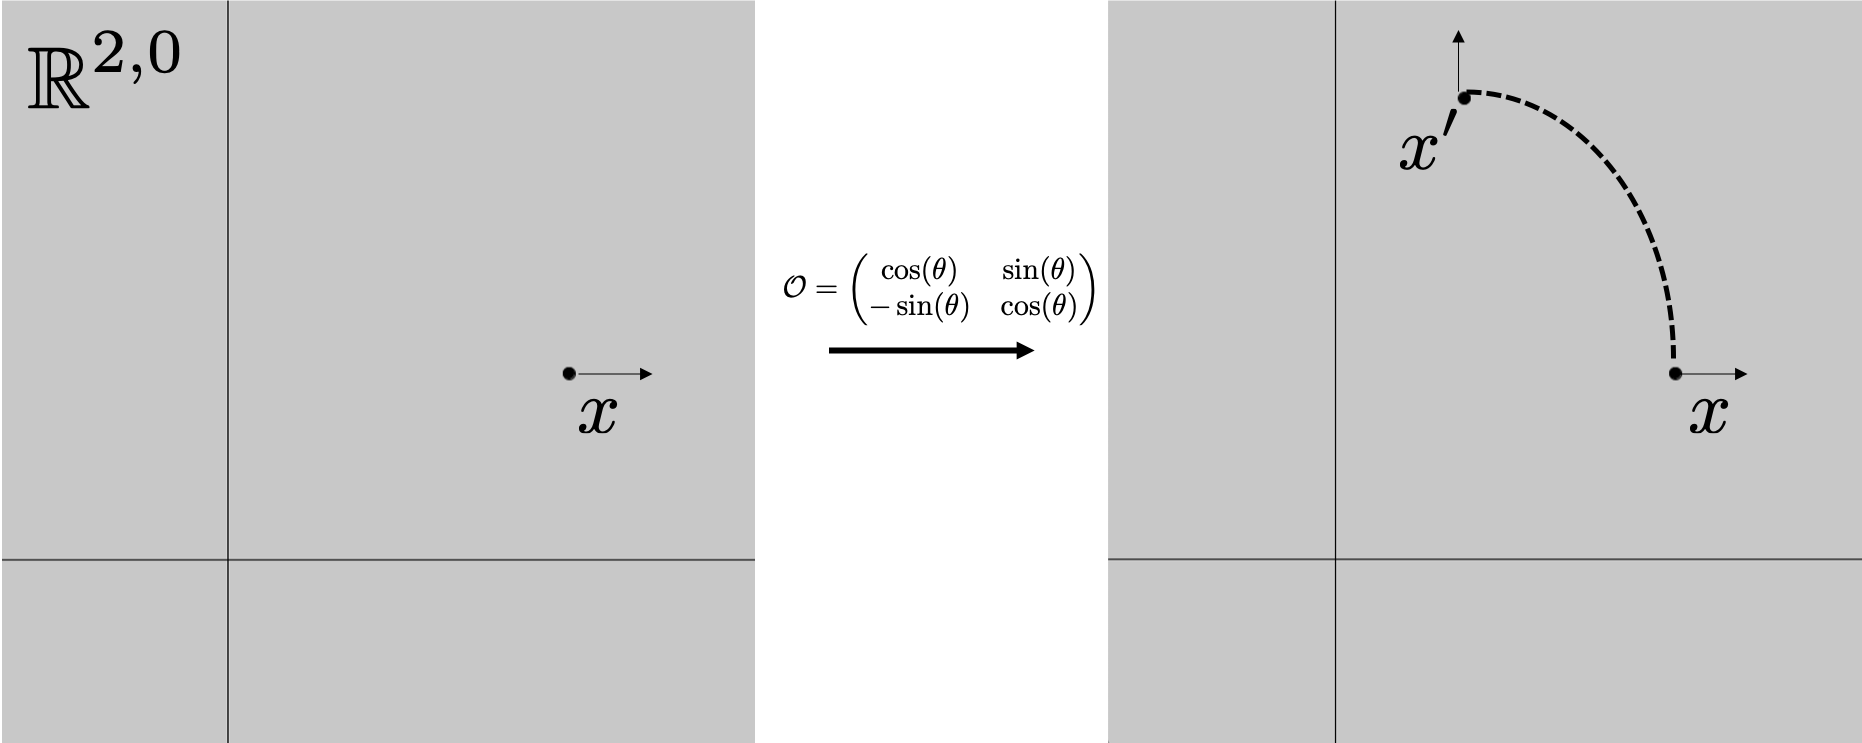
\includegraphics[width=4in]{images/active_rotation.png} 
\end{figure} 

\noindent After the rotation, the new field configuration at $x$ is

\begin{equation}
\phi'_a (x) = \sum_b \pi (\mathcal{O})_{ab} \phi_b (\mathcal{O}^{-1} x).
\end{equation}

\noindent The trivial representation of the field component $b$ would simply be the identity $\pi(\mathcal{O})_{ab} = \delta_{ab}$, and the fundamental, nontrivial representation is written

\begin{equation}
\pi (\mathcal{O})_{ab} = [ \mathcal{O} ] _{ab}.
\end{equation}

\noindent How does the action $S$ transform under a symmetry transformation?

\begin{equation}
S' = \int d^d x \, \Big{|} \text{det} \left( \frac{\partial x'^\mu}{\partial x^\nu} \right) \Big{|} \mathcal{L} \left( \mathcal{F} \left( \phi (x) \right), \frac{\partial x^\nu}{\partial x'^{\mu}} \partial_\nu \mathcal{F} \left( \phi (x) \right) \right)
\end{equation}

\noindent We also know that our theory is a conformal field theory, conformally invariant, conformally symemtric if the equations of motion are invariant. This is equivalent to the Lagrangian density transforming up to a total derivative

\begin{equation}
\mathcal{L}' = \mathcal{L} + \text{total derivative}.
\end{equation}

\noindent Now, let's study the infinitesimal generators of the conformal group $\text{Conf} ( \mathbb{R}^{p,q} )$.

\begin{itemize}
\item Translation
	\subitem $P_\mu = -i \partial_\mu$
\item Dilation
	\subitem $D = -i x^\mu \partial_\mu$
\item Rotation (Boost)
	\subitem $L_{\mu\nu} = i (x_\mu \partial_\nu - x_\nu \partial_\mu)$
\item Special Conformal
	\subitem $K_\mu = -i (2 x_\mu x'^\nu \partial_\nu - x^2 \partial_\mu)$
\end{itemize}

\noindent Work out the commutation relations to form a Lie algebra (\textbf{Exercise}).

\begin{align}
[D, P_\mu] &= i P_\mu \\
[D, K_\mu] &= -i K_\mu \\
[K_\mu, P_\nu] &= 2i (\eta_{\mu\nu} D - L_{\mu\nu} ) \\
[K_\rho, L_{\mu\nu}] &= i (\eta_{\rho\mu} K_\nu - \eta_{\rho\nu} K_\mu) \\
[P_\rho, L_{\mu\nu}] &= i (\eta_{\rho\mu} P_\nu - \eta_{\rho\nu} P_\mu ) \\
[L_{\mu\nu}, L_{\rho\sigma}] &= i (\eta_{\nu\rho} L_{\mu\sigma} + \eta_{\mu\sigma} L_{\nu\rho} - \eta_{\mu\rho} L_{\nu\sigma} - \eta_{\nu\sigma} L_{\mu\rho} )
\end{align}

\noindent And the rest commute. \\

\noindent Our task now is to find out which kinds of fields transform under the conformal group and give representations of the conformal group. We already know that a field transforming under $\text{Conf}(\mathbb{R}^{p,q})$, a general conformal transformation, transforms under the subgroup Poincar\'e, which is generated by translation $P_\mu$ and rotation $L_{\mu\nu}$, as

\begin{equation}
\phi_a (x) \rightarrow_{\text{Poincar\'e}} \sum_b \pi(\Lambda)_{ab} \phi_b (\Lambda^{-1}x).
\end{equation}

\noindent Let's focus on the subgroup of $\text{Conf}(\mathbb{R}^{p,q})$ which leave the orgin fixed: rotations, dilations, and SCTs. The infinitesimal generators of this subgroup form a subalgebra by exponentiation

\begin{equation}
\Lambda = e^{i \omega^\alpha G_\alpha}, \,\, \text{where } \omega^\alpha \text{ is infinitesimal.}
\end{equation}

\noindent The group element $G_\alpha$ can be $K_\mu$, $D$, or $L_{\mu\nu}$. At the origin, the Poincar\'e transformation  of the field looks like

\begin{equation}
\phi_a (x=0) \rightarrow \sum_b \pi (e^{i \omega^\alpha G_\alpha})_{ab} \phi_b (\Lambda^{-1} x = 0)
\end{equation}

\noindent Where the representation is, by Taylor expansion,

\begin{equation}
\pi(e^{i \omega^\alpha G_\alpha}) = \pi(\mathbb{I}) + i \omega^\alpha \pi(G_\alpha).
\end{equation}

\noindent Rename the representations of the generators (group elements)

\begin{align}
\pi(D) &= \tilde{\Delta} (\text{scaling dimension})\\
\pi(K_\mu) &= \kappa_\mu \\
\pi(L_{\mu\nu}) &= S_{\mu\nu} \, (\text{spin}).
\end{align}

\noindent The commutation of these representations are then

\begin{align}
[ \tilde{\Delta}, S_{\mu\nu} ] &= 0 \\
[ \tilde{\Delta}, \kappa_\mu ] &= -i \kappa_\mu \\
[ \kappa_\mu, \kappa_\nu ] &= 0.
\end{align}

\noindent Now, suppose that the generators $S_{\mu\nu}$ are irreducible representations, irreps, of the Lorentz group, the group that describes spin/helicity. By Schur's lemma (\textbf{Exercise}), we find that the scaling dimension is trivial, and, in turn, by the commuation relations, that all generators $\kappa_\mu$ are also trivial

\begin{equation}
\tilde{\Delta} \propto \mathbb{I} \implies -i \kappa_\mu = 0.
\end{equation}

\noindent Now use this fact to show how dilations act on the fields. The coordinates transform as

\begin{align}
x &\rightarrow \lambda x \\
x &\rightarrow \lambda^\epsilon \lambda^\epsilon \dots \lambda^\epsilon x
\end{align}

\noindent At the origin, the field transforms as

\begin{align}
\phi_a (x=0) \rightarrow&  (\mathbb{I} + i \epsilon \tilde{\Delta}) \dots (\mathbb{I} + i \epsilon \tilde{\Delta}) \phi_a (0) \\
&= \lambda^{i \tilde{\Delta}_a} \phi_a (0) \\
&= \lambda^{-\Delta_a} \phi_a (0)
\end{align}


\noindent Where we used the Taylor expansion of the infinitesimal $\epsilon$, and the last line uses $\tilde{\Delta} = i \Delta \mathbb{I}$, since Schur's lemma tells us that the scaling deimension is trivial. \\

\noindent So, every conformal field has a behavior under dilations, defined by the scaling dimension $\Delta_a$, with Jacobian

\begin{equation}
\Big{|} \frac{\partial x'}{\partial x} \Big{|} = \Lambda^{-\frac{d}{2}}, \text{ where } \Lambda = \lambda^{-2}.
\end{equation}

\noindent And the metric transforms under dilations as

\begin{equation}
g'_{\mu\nu} = \lambda^{-2} g_{\mu\nu}.
\end{equation}

\noindent Putting all this together, the field now transforms as 

\begin{equation}
\phi_a (x) \rightarrow \phi'_a (x') = \Big{|} \frac{\partial x'}{\partial x} \Big{|}^{-\frac{\Delta}{d}} \phi_a (x).
\end{equation}

\noindent Filling in the Jacobian, the new field in terms of the orignial field and the original spacetime location is

\begin{align}
\phi'_a (x) &= \sum_b \pi(\Lambda)_{ab} \phi_b (\Lambda^{-1} x) \\
&= \sum_b [ \lambda^{-\Delta}]_{ab} \phi_b (\Lambda^{-1} x) \\
&= \lambda^{-\Delta} \phi_a (\Lambda^{-1} x) \\
&= \lambda^{-\Delta} \phi_a (\lambda^{-1} x).
\end{align}

\noindent By the Baker-Campbell-Hausdorff (BCH) formula, we know how the new field looks at all spacetime lcoations, not just the origin (\textbf{Exercise})

\begin{align}
e^{i x^\rho P_\rho} D e^{-i x^\rho P_\rho} &= D + x^\nu P_\nu \\
&\implies D \phi_a (x) = (-i x^\nu \partial_\nu + \tilde{\Delta} ) \phi_a (x).
\end{align}

\noindent In the next lecture, we give this the quantum treatment, where we will look for unitary representations (self-adjoint operators), that are labelled by quantum numbers, such as spin, scaling dimension, and central charge. The central charge will require projective unitary representations.


\clearpage

\section*{Lecture 4: Constraints of Conformal Invariance on Quantum Field Theories}
\label{sec: lec4}


\noindent Recall that a scale transformation on a classical field is characterized per field, indexed by $a$, by the scaling dimension $\Delta_a$ in the mapping

\begin{equation}
\phi_a (x) \rightarrow \lambda^{-\Delta_a} \phi_a (x).
\end{equation}

\noindent We now make a move to study quantum fields, using the classical limit to check our results. So, suppose we have done all of the hard work of quantization and have a quantum field theory. \\

\noindent \textbf{Digression}: In $(1+1)$ dimensions, some approaches to quantization include

\begin{itemize}
\item Vertex operator algebras.
\item (Local) Algebraic QFT
	\subitem Top-down approach where one attaches an algebra of observables to each point in spacetime and then makes sense of it as a field theory.
\item Functors from $n$-Categories to Hilbert spaces: $n$Cat $\rightarrow$ Hilb (Segal).
\end{itemize}

\noindent  \textbf{Digression}: A main assumption of this course is that quantum field theories are a subset of quantum theories, although some schools argue that QFT is done via path integrals, which is not obviously a quantum theory. \\

\noindent The data of a quantum field theory includes

\begin{itemize}
\item Hilbert space of states $\mathcal{H}$
\item Projective unitary representation of the conformal group $U(g)$, where $g \in \text{Conf}(\mathbb{R}^{p,q})$
\item Vacuum (reference) state $\ket{0} \in \mathcal{H}$ \\
	\\ Invariant, up to a phase, under global symmetries, but not necessarily local symmetries: $U(g) \ket{0} = e^{i \varphi (g)} \ket{0}$. \\
	\\ If $p+q > 2$, then the global and local (full conformal) symmetries coincide. \\
	\\ If $p=q=1$, then the local conformal group of transformations (diffeomorphisms of the circle) is much larger than the global conformal group, making the global transformations subgroup of the local transformations. \\
\item Observables.
\end{itemize}

\noindent For observables, we demand that we can measure some set of local observables from the set of self-adjoint linear operators on the Hilbert space

\begin{equation}
A_{j,x} \in L_{\text{self-adjoint}} (\mathcal{H}); \,\, x \in \mathbb{R}^{p,q}; \,\, j \in \text{index set (e.g., particle type)}.
\end{equation}

\noindent \textbf{Digression}: We concern ourselves with \textit{local} observables, and non-local observables are difficult to imagine. An example of a non-local observable that shows up in gauge theory is the Wilson loop or Wilson line, since they are spread over a nonzero dimensional submanifold of the gauge theory's manifold. \\

\noindent Note that locality is induced by causality, such that if $x-y$ is spacelike, then $A_{j,x}$ and $A_{k,y}$ are jointly observable, $\forall \, j,k \text{ and } x,y$. \\

\subsection*{Quasi-Primary Observables}

\noindent The \textit{quasi-primary} of a field is a subset of local observables $\{ A_{j,x}: \, j \in J, x \in \mathbb{R}^{p,q} \}$ with the additional properties to satisfy the assumed constraints that enforce conformal invariance of the system, denoted here by $\{ \hat{\phi}_k (x): \, k \in K \}$ that transform as

\begin{equation}
U(g): \,\, \hat{\phi}_k (x) \rightarrow U^\dagger (g) \hat{\phi}_k (x) U(g) = \Big{|} \frac{\partial x'}{\partial x} \Big{|}^{\frac{\Delta_k}{d}} \hat{\phi}_k (x')
\end{equation}

\noindent Where $x' = gx$, and $g \in \text{Conf}(\mathbb{R}^{p,q})$ is a conformal transformation. \\

\noindent Now we must demonstrate that these assumptions yield nontrivial examples of fields. Rest assured that there are such fields, such as free bosons and free fermions. \\

\noindent By these assumptions, the $n$-point correlation function, which is observable via scattering experiments,  transforms under conformal transformations as

\begin{equation}
\bra{0} \hat{\phi}_{k_1} (x_1) \dots \hat{\phi}_{k_n} (x_n) \ket{0} = \Big{|} \frac{\partial x_1'}{\partial x_1} \Big{|}^{\frac{\Delta_{k_1}}{d}} \dots \Big{|} \frac{\partial x_n'}{\partial x_n} \Big{|}^{\frac{\Delta_{k_n}}{d}} \bra{0} \hat{\phi}_{k_1} (x'_1) \dots \hat{\phi}_{k_n} (x'_n) \ket{0}.
\end{equation}

\noindent This equation constrains the structure of the $n$-point correlation functions. To understand these constraints, let's analyze how each type of transformation of the conformal group constrains the invariants. \\

\noindent \textbf{Translations}: For $x_j, x_k \in \mathbb{R}^{p,q}$, $j, k = 1, \dots, n$, the difference $x_j - x_k$ is invariant, and there are $d(n-1)$ such quantities. \\

\noindent \textbf{Rotations}: For spinless objects (in large enough dimension $d$), the length $r_{jk} \equiv |x_j - x_k |$ is invariant, and there are ${n \choose 2}$ such quantities. \\

\noindent \textbf{Dilations}: Under the scale transformations, the length $r_{jk}$ is clearly not invariant, but the ratio $\frac{r_{jk}}{r_{lm}}$ can be invariant. \\

\noindent \textbf{SCTs}: Under special conformal transformations, invariant quantities must be cross ratios of the form $\frac{r_{jk} r_{lm}}{r_{jl} r_{km}}$, since the squared length under SCTs transforms as

\begin{equation}
|x'_1 - x'_2 |^2 = \frac{|x_1 - x_2 |^2}{(1 + 2 b \cdot x_1 + b^2 x_1^2) (1 + 2 b \cdot x_2 + b^2 x_2^2)}.
\end{equation}

\subsection*{Two-Point Correlation Functions}

\noindent Consider the classical two-point correlation function, or Green's function, of the quasi-primary fields

\begin{equation}
G^{(2)} (x_1, x_2) = \bra{0} \phi_1 (x_1) \phi_2 (x_2) \ket{0} = \Big{|} \frac{\partial x_1'}{\partial x_1} \Big{|}^{\frac{\Delta_{k_1}}{d}} \Big{|} \frac{\partial x_2'}{\partial x_2} \Big{|}^{\frac{\Delta_{k_2}}{d}} \bra{0} \hat{\phi}_{k_1} (x'_1) \hat{\phi}_{k_2} (x'_2) \ket{0}.
\end{equation}

\noindent Exploiting the assumed conformal symmetries of the system, use the fact that the Jacobian for a translation, as well as for a rotation, is equal to one, such that $\Big{|} \frac{\partial x'}{\partial x} \Big{|} = 1$, and, therefore, the Green's function can only depend on the length 

\begin{equation}
G^{(2)} (x_1, x_2) = f(|x_1 - x_2|) = f(r_{12}).
\end{equation}

\noindent For a dilation, the Jacobian obeys a scale factor, such that $\Big{|} \frac{\partial x'}{\partial x} \Big{|} = \lambda^{\Delta}$, and the Green's function has the form

\begin{equation}
G^{(2)} (x_1, x_2) = \lambda^{\Delta_1 + \Delta_2} f(\lambda r_{12}).
\end{equation}

\noindent To calculate the function that obeys this constraint, expand $f(r_{12}) = \sum_a f_a r_{12}^a$ in a series, noting that $a$ can be a continuous parameter, and compare to the above to get the condition that the coefficients $f_a$ are all zero, except for $a = -\Delta_1 - \Delta_2$. \\

\noindent Therefore, under translations, rotation, and dilations, we find that the Green's function is constrained to the form

\begin{equation}
G^{(2)} (x_1, x_2) = \frac{f_{-\Delta_1 - \Delta_2}}{r_{12}^{\Delta_1 + \Delta_2}} = \frac{c_{12}}{r_{12}^{\Delta_1 + \Delta_2}}
\end{equation}

\noindent Where $c_{12}$ is a constant determined by the normalization condition. \\

\noindent So far, we have come to the conclusion that the correlation function must obey a power law, and we now apply the constraints of SCTs to find that the two-point correlation function of quasi-primary fields is zero unless the two fields have the same scaling dimension $\Delta_1 = \Delta_2 = \Delta$ (\textbf{Exercise})

\begin{equation}
\bra{0} \phi_1 (x_1) \phi_2 (x_2) \ket{0} = \frac{c_{12}}{r_{12}^{2\Delta}}.
\end{equation}

\noindent This means that if we solve a system and the calculate the two-point correlation function of two fields with different scaling dimensions, $\Delta_1$ and $\Delta_2$, respectively, where $\Delta_1 \ne \Delta_2$, and get a nonzero result, then our system is not conformally invariant under the full global conformal group, but under a subgroup consisting of translations, rotations, and dilations. \\

\subsubsection*{Example: Three-Point Correlation}

\noindent Following similar procedure as in the two-point case, translations, rotations, and dilations lead to conclusion that the three-point correlation function must have the form

\begin{equation}
\bra{0} \phi_1 (x_1) \phi_2 (x_2) \phi_3 (x_3) \ket{0} = \sum_{a,b,c} \frac{c_{abc}}{r_{12}^a r_{23}^b r_{31}^c}
\end{equation}

\noindent Where the summation is constrained by the field scaling dimensions to satisfy $a+b+c = \Delta_1 + \Delta_2 + \Delta_3$. \\

\noindent Special conformal transformations further constrain the exponents in the power law to (\textbf{Exercise})

\begin{equation}
a = \Delta_1 + \Delta_2 - \Delta_3, \,\,\,\, b = -\Delta_1 + \Delta_2 + \Delta_3, \,\,\,\, c = \Delta_1 - \Delta_2 + \Delta_3.
\end{equation}

\noindent And the three-point correlation function has the form

\begin{equation}
\bra{0} \phi_1 (x_1) \phi_2 (x_2) \phi_3 (x_3) \ket{0} = \frac{c_{123}}{r_{12}^{\Delta_1 + \Delta_2 - \Delta_3} r_{23}^{-\Delta_1 + \Delta_2 + \Delta_3} r_{31}^{\Delta_1 - \Delta_2 + \Delta_3}}.
\end{equation}

\subsubsection*{Example: Four-Point Correlation}

\noindent The four-point correlation function has the form

\begin{equation}
\bra{0} \phi_1 (x_1) \phi_2 (x_2) \phi_3 (x_3) \phi_4 (x_4) \ket{0} = F \left( \frac{r_{12} r_{34}}{r_{13} r_{24}}, \frac{r_{13} r_{24}}{r_{23} r_{14}} \right) \prod_{j<k} r_{jk}^{-\Delta_j - \Delta_k + \frac{\Delta}{3}}
\end{equation}

\noindent Where $F(\cdot,\cdot)$ is an arbitrary function of the cross products and $\Delta = \sum_j \Delta_j$.

\subsection*{Conformal Theory in $(2+0)$ Dimensions}

\noindent Thus far, we have been studying the structure of conformal theories in arbitrary spacetime dimension $d$. In $(2+0)$ dimensions, conformal theories will take on a new definition. \\

\noindent Recall that we defined the complex fields $z = x_1 + i x_2$ and $\bar{z} = x_1 - i x_2$, and made the assumption that we can \textit{analytically continue} to arbitrary, independent $z$ and $\bar{z}$, such that

\begin{equation}
\Phi(x_1,x_2) = \Phi(z,\bar{z})
\end{equation}

\noindent And work out the consequences from there. We now extend our definition of quasi-primary fields, by analogy to the general, arbitrary dimension case. We will now refer to these fields as \textit{primary fields} of type, or conformal weight, $(h, \bar{h})$ with the proposed form

\begin{equation}
\Phi (z, \bar{z}) = \left( \frac{\partial f}{\partial z} \right)^h \left( \frac{\partial \bar{f}}{\partial \bar{z}} \right)^{\bar{h}} \Phi (f(z), \bar{f} (\bar{z})).
\end{equation}

\noindent Note here that there are indeed enough examples of primary fields of conformal field theories to make these assumptions interesting to study. \\

\noindent Expand the primary field infinitesimally, as it is the more convenient method opposed to working with the full global transformation, by sending $z \rightarrow z + \epsilon(z)$, and complex conjugate, to order $\epsilon$

\begin{equation}
\delta_{\epsilon, \bar{\epsilon}} \Phi (z, \bar{z}) = ((h \partial_z \epsilon(z) + \epsilon (z) \partial_z ) + (\bar{h} \partial_{\bar{z}} \bar{\epsilon}(\bar{z}) + \bar{\epsilon} (\bar{z}) \partial_{\bar{z}} )) \Phi(z, \bar{z}).
\end{equation}

\noindent And write the two-point correlation function as

\begin{equation}
G^{(2)} (\underline{z}, \bar{\underline{z}}) = \bra{0} \Phi_1 (z_1, \bar{z}_1) \Phi_2 (z_2, \bar{z}_2) \ket{0}
\end{equation}

\noindent Where $\underline{z} \equiv (z_1, z_2)$ and $\underline{\bar{z}} \equiv (\bar{z}_1, \bar{z}_2)$. \\

\noindent Applying the infinitesimal equation for $\delta_{\epsilon, \bar{\epsilon}} \Phi (z, \bar{z})$ from above, and setting equal to zero by conformal invariance to order $\epsilon$, we get

\begin{equation}
\delta_{\epsilon, \bar{\epsilon}} G^{(2)} (\underline{z}, \underline{\bar{z}}) = \bra{0} \delta_{\epsilon, \bar{\epsilon}} \Phi_1 \Phi_2 \ket{0} + \bra{0} \Phi_1 \delta_{\epsilon, \bar{\epsilon}} \Phi_2 \ket{0} = 0.
\end{equation}

\noindent From here, as before in the arbitrary dimension case, we can work out the constraints of each type of conformal transformation on the correlation function. \\

\noindent \textbf{Translation}: 

\begin{equation}
\epsilon(z) = \epsilon \implies G^{(2)}(\underline{z}, \underline{\bar{z}}) \propto z_{12} = z_1 - z_2 \text{ and }\bar{z_{12}} = \bar{z}_1 - \bar{z}_2.
\end{equation}

\noindent \textbf{Rotation \& Dilation}: 

\begin{equation}
\epsilon (z) = \epsilon z \implies G^{(2)}(\underline{z}, \underline{\bar{z}}) = \frac{c_{12}}{z_{12}^{h_1 + h_2} \bar{z}_{12}^{\bar{h}_1 + \bar{h}_2}}.
\end{equation}

\noindent \textbf{SCT}: 

\begin{equation}
\epsilon (z) = z^2 \implies G^{(2)}(\underline{z}, \underline{\bar{z}}) = \frac{c_{12}}{z_{12}^{2h} \bar{z}_{12}^{2\bar{h}}}.
\end{equation}

\noindent Now, for example, suppose we have a bosonic field which applies the constraint $h-\bar{h}=0$ to the conformal weights. Setting $h+\bar{h} = \Delta$, the analytically continued two-point correlation function for the bosonic field becomes

\begin{equation}
G^{(2)}(\underline{z}, \underline{\bar{z}}) = \frac{c_{12}}{|z_{12}|^{2\Delta}}.
\end{equation}

\subsubsection*{Example: Three-Point Correlation}

\noindent Similarly, the three-point correlation function has the form

\begin{equation}
G^{(3)} (\underline{z}, \underline{\bar{z}}) = c_{123} \frac{1}{z_{12}^{h_1+h_2-h_3} z_{23}^{-h_1+h_2+h_3} z_{31}^{h_1-h_2+h_3}} \frac{1}{\bar{z}_{12}^{h_1+h_2-h_3} \bar{z}_{23}^{-h_1+h_2+h_3} \bar{z}_{31}^{h_1-h_2+h_3}}
\end{equation}

\noindent In summary, we have introduced what we consider quantum field theories and have analyzed the consequences of conformal invariance of these quantum theories. We have also analyzed subclasses of theories that obey additional constraints (e.g., $\Delta = h + \bar{h}$ is real).

\clearpage

\section*{Lecture 5: \\ Quantum CFT: Ward Identities \& Radial Quantization}
\label{sec: lec5}

%
\noindent We have been on this journey from classical conformal symmetries to the implementation of the symmetries in a quantum setting. Thus far, we have found that the constraints of conformal symmetry in the context of quantum field theory, in $(2+0)$, $(1+1)$, and $(d+1)$ dimensions, the two-point correlation functions must decay polynomially as

\begin{equation}
\bra{0} \hat{\phi} (x) \hat{\phi} (y) \ket{0} \propto \frac{1}{|x-y|^\alpha}.
\end{equation}

\subsection*{Radial ``Quantization''}

\noindent Note that using quotes around quantization indicates that this approach is an inspired guess, and is not derived via a functor. \\

\noindent To build a quantum field theory with conforml symmetry, invariant under the group Conf$(\mathbb{R}^{2,0})$, we need four pieces of data. \\

\noindent (1) We need a Hilbert space $\mathcal{H}$ which is preferrably an infinite, separable, kinematic space of states isomorphic to the vector space of linear operators $L^2 (\mathbb{R})$, (2) a vacuum state, or a reference vector, $\ket{0}$, a subset of linear operators in the Hilbert space $\mathcal{L}(\mathcal{H})$ called \textit{observables} $\hat{\phi} (x,y)$, $(x,y) \in \mathbb{R}^2$, which are distribution-valued objects, but can be thought of, without harm, as self-adjoint operators. \\

\noindent The choice of set of observables, the subset of linear operators from the Hilbert space, define and distinguish a quantum field theory from others. E.g., the bosonic quantum field and the hydrogen atom share the same Hilbert space, but their observables are different and define what is allowed to be measured in each quantum field theory. \\

\noindent Our conformal quantum field theory yields (projective) unitary representations of Conf$(\mathbb{R}^{2,0})$. We can use analytic continuation to map to a Minkowski theory where we have representations of Conf$(\mathbb{R}^{1,1})$. \\

\noindent Introduce the construction of ``imaginary time''

\begin{equation}
\begin{pmatrix} x \\ y \end{pmatrix} \rightarrow \begin{pmatrix} x \\ it \end{pmatrix}; \,\, t \in \mathbb{R}.
\end{equation}

\noindent If possible, the correlation functions analytically continue, such that

\begin{equation}
\bra{0} \hat{\phi} (x,y) \hat{\phi} (0,0) \ket{0} = f(x,y) \rightarrow f(x,it).
\end{equation}

\noindent If all $n$-point correlation functions are analytically continued in this way, it \textit{often} happens that we get a mapping

\begin{equation}
G^{(n)} ((x_1,y_1), \dots) \rightarrow G^{(n)} ((x_1,t_1), \dots)
\end{equation}

\noindent Which are invariant, respectively, under symmetry transformations

\begin{equation}
\text{Conf}(\mathbb{R}^{2,0}) \rightarrow \text{Conf}(\mathbb{R}^{1,1}).
\end{equation}

\noindent This is the analytic continuation to a \textit{Minkowski theory}, and the criteria to ensure that this mapping exists is called \textit{reflection positivity}. See the work of Glimm and Jaffe for a rigorous account of this machinery. \\

\noindent With a Minkowski quantum field theory, enter the Heisenberg picture to apply time evolution, and analytically continue the ``time'' variable to define ``inverse temperature'' $t \rightarrow -i\beta$, which essentially gives the correlation function for the thermal state of the Hamiltonian $\hat{H}$ with inverse temperature $\beta$

\begin{align}
\bra{0} \hat{\phi} (x,y) \hat{\phi} (0,0) \ket{0} &= \bra{0} e^{-it \hat{H}} \hat{\phi} (x,0) e^{it\hat{H}} \hat{\phi} (0,0) \ket{0} \\
&= \bra{0} e^{-\beta \hat{H}} \hat{\phi} (x,0) e^{\beta \hat{H}} \hat{\phi} (0,0) \ket{0}.
\end{align}

\noindent \textbf{Digression}: What does ``physical'' mean for this course? \\

\noindent To define a physical theory, we require \textit{kinematics} and \textit{observables}, which make for a perfectly fine physical theory, even without \textit{dynamics}. \\

\noindent The kinematics of a system introduces a Hilbert space $\mathcal{H}$ and a set of density operators $\rho(\mathcal{H})$ that describe the states of the system, but do not allow measurement of those states. The observables of a system $\mathcal{O} \subset \mathcal{L}(\mathcal{H})$ are the measurements of the states of the system, and are labelled by points in the underlying manifold $\mathcal{M}$ of the theory, such that $x, x^\dagger, \mathbb{I} \in \mathcal{O}, \, \text{ for } x \in \mathcal{M}$. \\

\noindent Dynamics of a system are introduced via the group of isometries on the manifold $G = \text{Isom}(\mathcal{M})$, and, for a quantum field theory, we search for projective, unitary representations of $G$ on the Hilbert space. The construct of time only comes in as a choice of the manifold and its one-dimensional subgroups that act like time, but time is not necessarily an axiom of a quantum theory. \\

\noindent \textbf{End Digression}. \\

\noindent So far, we have labelled our observables in our Minkowski CFT by $(\sigma^0, \sigma^1) \in \mathbb{R}^{1,1}$. We now complexify these coordinates by ``Euclideanizing'' and sending the timelike coordinate to be imaginary, such that $\sigma^0 \rightarrow i \sigma^0$, and 

\begin{equation}
z = \sigma^1 + i \sigma^0 \text{ and } \bar{z} = \sigma^1 - i \sigma^0
\end{equation}

\noindent Which correspsonds to an analytic continuation of the $n$-point correlation functions

\begin{equation}
G^{(n)} (\underline{\sigma}_1, \underline{\sigma}_2, \dots) \rightarrow G^{(n)} (\underline{z}_1, \bar{\underline{z}}_1; \underline{z}_2, \bar{\underline{z}}_2; \dots).
\end{equation}

\noindent In this complexifed, Euclidean spacetime, with locations defined by coordinates $z$ and $\bar{z}$, compactify space to a cylinder, such that space corresponds to the transverse direction $\sigma^1 \rightarrow \sigma^1 + 2\pi$, and time corresponds to the longitudinal direction, and our complex coordinates are now

\begin{equation}
z = e^{\sigma^1 + i \sigma^0} \text{ and } \bar{z} = e^{\sigma^1 - i \sigma^0}.
\end{equation}

\noindent Circles in the complex plane correspond to constant time, the radial direction on the cylinder, and the real coordinates $\sigma^0, \sigma^1$ are mapped to the complex coordinates as

\begin{equation}
\sigma^0 = \infty \rightarrow z = \infty \text{ and  } \sigma^0 = -\infty \rightarrow z=0
\end{equation}

\noindent And transformations maps as

\begin{align}
\text{Time reversal } [\sigma^0 \rightarrow -\sigma^0] &\rightarrow \text{Inversion } [z \rightarrow \frac{1}{z}] \\
\text{Time translation } [\sigma^0 \rightarrow \sigma^0 + a] &\rightarrow \text{Dilation } [z \rightarrow e^a z] \\
\text{Spatial translation } [\sigma^1 \rightarrow \sigma^1 + a] &\rightarrow \text{Rotation } [z \rightarrow e^{ia} z] 
\end{align}

\begin{figure}[H]
	\centering
	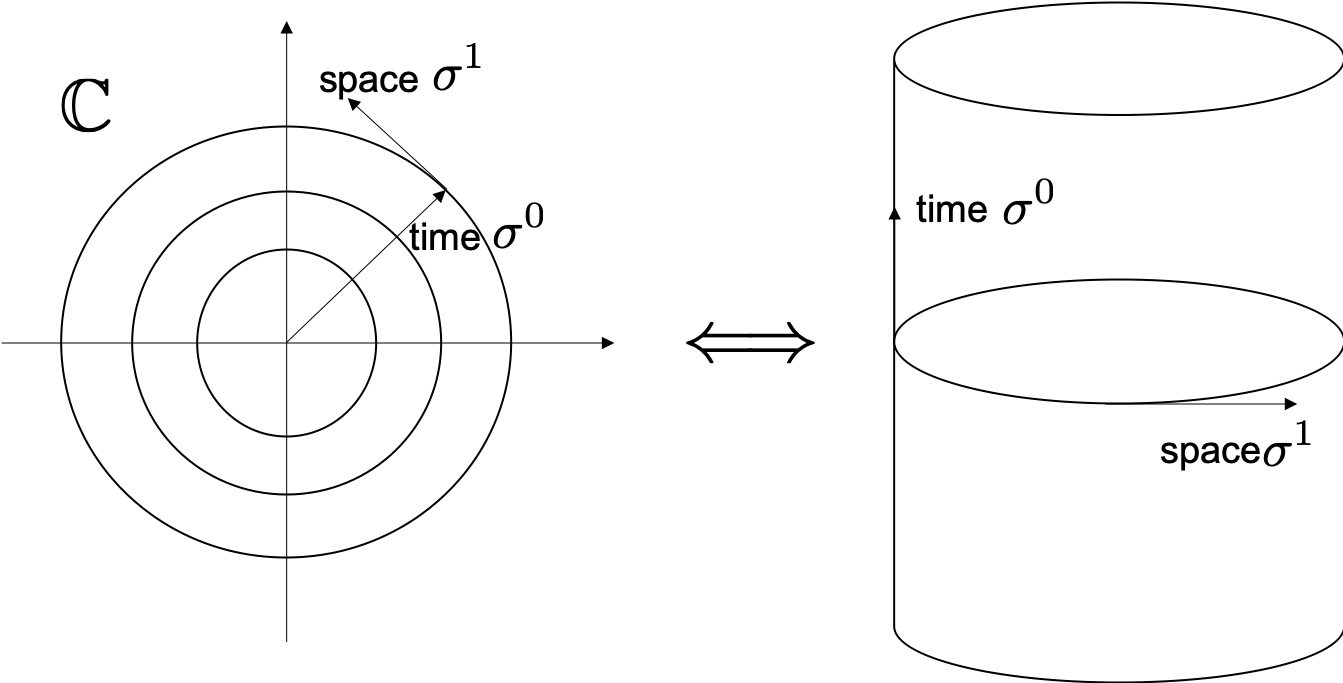
\includegraphics[width=3.5in]{images/radial_quantization.png} 
\end{figure} 

\noindent Now we make a move to constructing a conformal field theory in complexified, Euclidean spacetime. \\

\subsection*{Ward Identities}

\noindent Witha conformally invariant classical theory, we work towards getting a collection of observables obeying the correct symmetry for a conformally invariant quantum theory. \\

\noindent Recall from Noether's theorem that conserved charges correspond to classical symmetries $Q$ obeying the anticommutation bracket

\begin{equation}
\{ Q_j, Q_k \} = f_{jk}^{\,\,\,\,l} Q_l.
\end{equation}

\noindent We may try to naively quantize by ``puttings hats on'' the conserved quantities that obey the commutation brackets

\begin{equation}
[ \hat{Q}_j, \hat{Q}_k ] = i f_{jk}^{\,\,\,\,l} \hat{Q}_l,
\end{equation}

\noindent But without a Hilbert space, we can not write these operators as functions of the fields (e.g., $\hat{Q} = f(\hat{\phi})$. \\

\noindent From the classical symmetries, we now derive the quantum generators of the symmetries. \\

\noindent Suppose we have a classical field theory with action $S[\underline{\phi}]$, where $\underline{\phi}$ is a vector of classical fields. Assume that $S$ is symmetric under the Lie group of infinitesimal transformations, such that

\begin{equation}
\underline{\phi}' (\underline{x}) = \underline{\phi} (\underline{x}) - i \omega_a (\underline{x}) \textbf{G}_a \underline{\phi} (\underline{x}) = e^{-i \omega_a (\underline{x}) \textbf{G}_a} \underline{\phi} (\underline{x})
\end{equation}

\noindent Where $\omega_a (\underline{x})$ is infinitesimal and $\textbf{G}_a$ is a matrix acting on the vector labels of $\underline{\phi}$. \\

\noindent Use the path integral prescription to work out how this transformation affects the correlation functions

\begin{equation}
\bra{0} \underline{\hat{\phi}} (\underline{x}_1) \dots \underline{\hat{\phi}} (\underline{x}_n) \ket{0} = \lim_{T \rightarrow \infty(1-i\epsilon)} \frac{\int \mathcal{D}\phi \, \phi (\underline{x}_1) \dots \phi (\underline{x}_n) e^{iS[\underline{\phi}]}}{\int \mathcal{D} \phi \, e^{i S[\underline{\phi}]}}.
\end{equation}

\noindent The first step is to change variables $\underline{\phi} \rightarrow \underline{\phi}'$ and assume that the measure is invariant $\mathcal{D}\phi' = \mathcal{D}\phi$. Define the operator $\hat{X}$ to be the time-ordered product of quantum fields

\begin{equation}
\hat{X} = \mathcal{T} [ \underline{\hat{\phi}} (\underline{x}_1) \dots \underline{\hat{\phi}} (\underline{x}_n)].
\end{equation}

\noindent Note that the time-ordering will be assumed from here on, and consider the expectation value of $\hat{X}$ in the path integral prescription

\begin{equation}
\langle \hat{X} \rangle = \frac{\int \mathcal{D} \phi' \, \left( \underline{\hat{\phi}} (\underline{x}_1) \dots \underline{\hat{\phi}} (\underline{x}_n) + i \omega_a (\underline{x}) \textbf{G}_a (\underline{\hat{\phi}} (\underline{x}_1) \dots \underline{\hat{\phi}} (\underline{x}_n) + \dots \right) e^{i (S + \int dx \, \partial_\mu j_a^\mu \omega_a (\underline{x}))}}{\int \mathcal{D}\phi \, e^{iS}}.
\end{equation}

\noindent To zeroth order in $\omega_a$, this is exactly the correlation function prior to the change of variables. To first order in $\omega_a$, we get the equality for quantum fields

\begin{equation}
\frac{\partial}{\partial x^\mu} \langle \hat{j}_a^\mu (\underline{x}) \hat{\phi} (\underline{x}_1) \dots \hat{\phi} (\underline{x}_n) \rangle = -i \sum_{j=1}^{n} \delta(\underline{x} - \underline{x}_j) \langle \hat{\phi} (\underline{x}_1) \dots \textbf{G}_a \hat{\phi} \left( \underline{x}_j) \dots \hat{\phi} (\underline{x}_n) \right)\rangle.
\end{equation}

\noindent The generator of symmetry $\hat{j}_a^\mu (\underline{x})$ is handed over by the oath integral approach.

%\clearpage

\end{document}